% ============================================================
%  Kit de la clínica (Clase 23): informe técnico de Cafés Altavista
%  Pronóstico de ventas diarias por tienda
%  Curso: Análisis y Visualización de Datos para la Toma de Decisiones
%
%  Es el insumo para quien no tiene un caso propio: un informe escrito, a
%  propósito, en lenguaje técnico y sin recomendación. La actividad es
%  convertirlo en un pitch de cinco minutos para la gerencia.
%
%  Datos y figuras: ../../../scripts/semana12-clase23_kit.py, a partir de
%  cafes_altavista.xlsx (Clase 16). Todas las cifras salen de ese script.
%  Compilar con: xelatex informe-tecnico-kit.tex (dos veces)
% ============================================================
\documentclass[11pt]{article}

\usepackage[a4paper,margin=2cm]{geometry}
\usepackage{fontspec}
\usepackage{amsmath}
\usepackage[spanish,es-noshorthands,es-tabla]{babel}
\usepackage{xcolor}
\usepackage{graphicx}
\usepackage{booktabs}
\usepackage{array}
\usepackage{tabularx}
\usepackage{enumitem}
\usepackage{fancyvrb}
\usepackage{tcolorbox}
\usepackage{fancyhdr}
\usepackage{hyperref}

\IfFontExistsTF{Aptos}{\setmainfont{Aptos}}{\setmainfont{Lato}}
\setmonofont{DejaVu Sans Mono}[Scale=0.82]

\definecolor{esumerNavy}{HTML}{262E66}
\definecolor{esumerNavyDark}{HTML}{1E4093}
\definecolor{esumerTeal}{HTML}{0CB3B6}
\definecolor{esumerOrange}{HTML}{EF7C2C}
\definecolor{esumerBg}{HTML}{F7F8FA}

\hypersetup{colorlinks=true, linkcolor=esumerNavyDark, urlcolor=esumerNavyDark}
\graphicspath{{figuras/}{../../../plantilla/assets/}}

\newcommand{\urldatos}{https://github.com/craljimenez/An-lisis_y_Visualizacion_de_Datos_para_la_Toma_de_Decisiones/raw/main/clases/semana12-clase23-clinica-analitica-storytelling/datos/ventas_diarias_tiendas.csv}

\pagestyle{fancy}
\fancyhf{}
\renewcommand{\headrulewidth}{0pt}
\fancyfoot[L]{\small\color{esumerNavyDark} Kit de la clínica \textperiodcentered\ Clase 23}
\fancyfoot[R]{\small\color{esumerNavyDark} \thepage}
\setlength{\parindent}{0pt}
\setlength{\parskip}{4pt}
\setlength{\emergencystretch}{1.5em}
\fvset{fontsize=\small}

\newcommand{\seccion}[1]{\par\vspace{6pt}{\large\bfseries\color{esumerNavy} #1}\par\vspace{1pt}}

\begin{document}

% ---------------- Portada de instrucciones ----------------
\begin{minipage}[c]{0.18\textwidth}
  \includegraphics[height=1.15cm,width=\linewidth,keepaspectratio]{esumer-logo.png}
\end{minipage}%
\begin{minipage}[c]{0.80\textwidth}
  \raggedleft
  {\Large\bfseries\color{esumerNavy} Kit de la clínica: el caso de Cafés Altavista}\\[3pt]
  {\small\color{esumerNavyDark} Semana 12 \textperiodcentered\ Clase 23 \textperiodcentered\ Insumo para la actividad}
\end{minipage}

\vspace{4pt}
{\color{esumerOrange}\rule{\textwidth}{2pt}}
\vspace{4pt}

\begin{tcolorbox}[colback=esumerBg, colframe=esumerTeal, boxrule=0.6pt, arc=1mm,
  title=Para qué es este kit, fonttitle=\bfseries\small, colbacktitle=esumerTeal,
  left=6pt, right=6pt, top=3pt, bottom=3pt]
\small Si no tienes un caso propio con un modelo, o no hiciste las
actividades de las Clases 20 a 22, usa este. En las páginas siguientes está
el \textbf{informe técnico} que el equipo de analítica de Cafés Altavista (la
empresa de la Clase 16) le entregó a la gerencia.

El informe está bien hecho, pero está escrito \textbf{para analistas}:
habla de MAE, $R^2$ y coeficientes, y \textbf{no dice qué hacer}. Tu trabajo
en la clínica es convertirlo en un \textbf{pitch de cinco minutos para la
gerencia}, como en el ejemplo de las bicicletas.
\end{tcolorbox}

\seccion{Lo que tienes que hacer}

\begin{enumerate}[itemsep=3pt, topsep=2pt]
  \item \textbf{Lee el informe} (15 minutos) y subraya las cifras que le
    importarían a la gerencia.
  \item \textbf{Traduce el modelo} con la tabla ``El modelo, sin jerga'' de la
    clase: ¿qué predice?, ¿con qué?, ¿qué tan bien frente a hoy?, ¿qué
    aprendió?
  \item \textbf{Encuentra el hallazgo} que lleva a una decisión. Pista: está
    en la figura de la sección 3.
  \item \textbf{Propón una recomendación}: qué, quién, cuándo, qué esperas y
    qué pides hoy. El informe no la trae: la decides tú, con los datos.
  \item \textbf{Escribe las limitaciones} en lenguaje de negocio (sección 5).
  \item \textbf{Arma el guion} de cinco diapositivas y \textbf{preséntalo} en
    la clínica.
\end{enumerate}

\seccion{Preguntas que te ayudan}

\begin{itemize}[itemsep=2pt, topsep=2pt]
  \item ¿Qué decisión diaria de la empresa usaría este pronóstico? Piensa en
    el personal de cada turno y en la panadería que se hornea cada mañana.
  \item ¿Qué tienda se comporta distinto a las demás los fines de semana?
    ¿Por qué podría ser?
  \item ``78 mil pesos de error por tienda y día'': ¿es mucho o poco? ¿Frente
    a qué?
  \item ¿Qué dato le falta al informe para poner el impacto en pesos? Dilo
    en tu presentación (Clase 22).
  \item ¿Qué no debe hacerse con este modelo?
\end{itemize}

\seccion{Si quieres explorar los datos}

El archivo
\href{\urldatos}{\color{esumerOrange}\texttt{ventas\_diarias\_tiendas.csv}}
tiene una fila por tienda y día, con las mismas columnas del informe. Puedes
abrirlo en Excel, Power BI, Python u Orange para hacer tus propios gráficos.
No es obligatorio: con el informe basta para la actividad.

\vspace{4pt}
{\footnotesize\itshape Cafés Altavista es una empresa ficticia y los datos son
simulados con fines académicos (Clase 16).}

% ============================================================
\clearpage
\begin{center}
{\Large\bfseries\color{esumerNavy} Informe técnico: pronóstico de ventas diarias por tienda}\\[4pt]
{\small Cafés Altavista S.A.S. \textperiodcentered\ Equipo de analítica \textperiodcentered\ Para: Gerencia general}
\end{center}
{\color{esumerNavy}\rule{\textwidth}{0.8pt}}

\seccion{1. Objetivo y datos}

Se estimó un modelo de regresión lineal (mínimos cuadrados ordinarios) para
pronosticar la venta neta diaria de cada tienda. La unidad de análisis es
tienda-día. Se agregaron las líneas de venta limpias (sin las 20 líneas
duplicadas del 20 de mayo y con los descuentos vacíos imputados en 0) del
1 de octubre de 2025 al 30 de septiembre de 2026: \textbf{2005 registros}.
Usaquén aporta 183 días (abrió el 1 de abril de 2026) y Granada 362 (sin
registros del 14 al 16 de julio).

\small
\renewcommand{\arraystretch}{1.12}
\begin{tabularx}{\textwidth}{@{}>{\raggedright\arraybackslash}p{4.3cm} >{\raggedright\arraybackslash}X@{}}
\toprule
\textbf{Variable} & \textbf{Definición}\\
\midrule
\texttt{ventas} & Variable dependiente: venta neta del día, en pesos.\\
\texttt{tienda} & Variable categórica, codificada con 5 variables indicadoras (referencia: Pereira Centro).\\
\texttt{fin\_de\_semana} & 1 si el día es sábado o domingo.\\
\texttt{diciembre} & 1 si el día es de diciembre de 2025.\\
\texttt{campana\_grano} & 1 si el día es de septiembre de 2026 (descuento de 25\% en café en grano).\\
\texttt{meses\_desde\_inicio} & Tendencia: 0 en octubre de 2025, 11 en septiembre de 2026.\\
\texttt{finde\_chapinero} & Interacción: \texttt{fin\_de\_semana} $\times$ (tienda = Chapinero).\\
\texttt{finde\_medellin} & Interacción: \texttt{fin\_de\_semana} $\times$ (tienda = El Poblado o Laureles).\\
\bottomrule
\end{tabularx}\par
\renewcommand{\arraystretch}{1.0}
\normalsize

\seccion{2. Metodología}

\begin{itemize}[itemsep=1pt, topsep=1pt]
  \item Partición aleatoria 80/20 con \texttt{train\_test\_split(test\_size=0.2,
    random\_state=42)}: 1604 registros de entrenamiento y 401 de prueba.
  \item \textbf{Línea base}: el promedio histórico de cada tienda, calculado en
    el entrenamiento. Es el método con el que hoy cada tienda planea su
    operación diaria.
  \item \textbf{Modelo 1}: tienda, \texttt{fin\_de\_semana}, \texttt{diciembre},
    \texttt{campana\_grano} y \texttt{meses\_desde\_inicio}.
  \item \textbf{Modelo 2}: el Modelo 1 más las interacciones
    \texttt{finde\_chapinero} y \texttt{finde\_medellin}, incorporadas tras el
    análisis de residuos del Modelo 1 (sección 3).
  \item Métricas sobre el conjunto de prueba: MAE (en pesos) y $R^2$.
\end{itemize}

\seccion{3. Análisis de residuos del Modelo 1}

En el Modelo 1, el coeficiente de \texttt{fin\_de\_semana} resultó cercano a
cero (3761). Sin embargo, el residuo promedio en los días de prueba presentó
un patrón sistemático por tienda: en Chapinero, $+71.000$ entre semana y
$-124.000$ en fin de semana; en El Poblado, $-31.000$ y $+93.000$. El efecto
del fin de semana tiene signo opuesto según la tienda y se cancela en el
coeficiente agregado. La figura muestra el promedio de ventas diarias de los
2005 registros:

\begin{center}
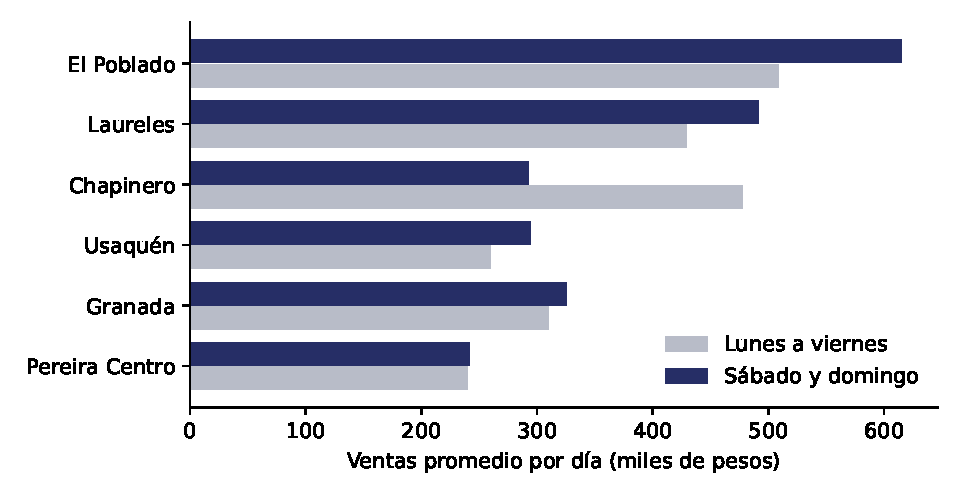
\includegraphics[width=0.78\textwidth]{kit_finde.pdf}
\end{center}

Variación de las ventas promedio del fin de semana frente a los días hábiles:
El Poblado $+21{,}0\%$, Laureles $+14{,}5\%$, Usaquén $+13{,}3\%$, Granada
$+5{,}2\%$, Pereira Centro $+0{,}8\%$ y Chapinero $-38{,}9\%$.

% ============================================================
\seccion{4. Resultados}

\begin{center}
\small
\renewcommand{\arraystretch}{1.15}
\begin{tabular}{@{}lrr@{}}
\toprule
\textbf{Especificación} & \textbf{MAE (pesos)} & \textbf{$R^2$}\\
\midrule
Línea base (promedio por tienda) & 92.420 & 0,436\\
Modelo 1 & 86.335 & 0,521\\
Modelo 2 & 78.039 & 0,603\\
\bottomrule
\end{tabular}

\vspace{4pt}
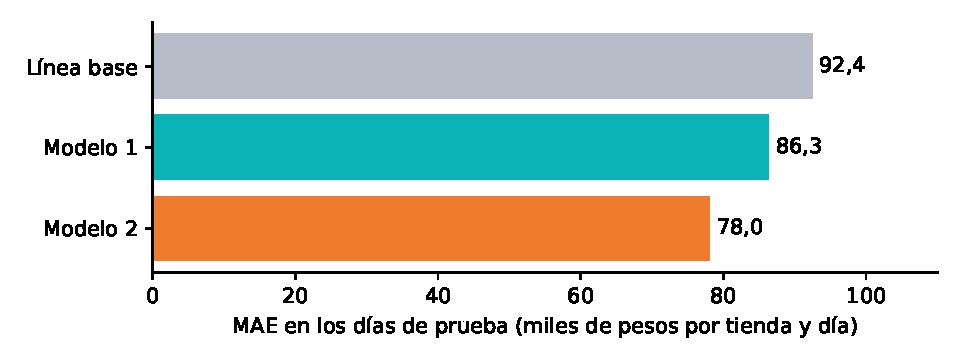
\includegraphics[width=0.7\textwidth]{kit_modelos.pdf}
\end{center}

El Modelo 2 reduce el MAE en 14.381 pesos por tienda-día frente a la línea
base ($-15{,}6\%$). Coeficientes estimados del Modelo 2 (intercepto: 173.898):

\begin{center}
\small
\renewcommand{\arraystretch}{1.1}
\begin{tabular}{@{}lr@{\hspace{1.5cm}}lr@{}}
\toprule
\textbf{Variable} & \textbf{Coeficiente} & \textbf{Variable} & \textbf{Coeficiente}\\
\midrule
\texttt{fin\_de\_semana} & 13.476 & \texttt{tienda\_El Poblado} & 276.921\\
\texttt{diciembre} & 119.779 & \texttt{tienda\_Chapinero} & 236.619\\
\texttt{campana\_grano} & 103.123 & \texttt{tienda\_Laureles} & 185.506\\
\texttt{meses\_desde\_inicio} & 8.108 & \texttt{tienda\_Granada} & 75.738\\
\texttt{finde\_chapinero} & $-194.464$ & \texttt{tienda\_Usaquén} & $-7.387$\\
\texttt{finde\_medellin} & 70.871 & & \\
\bottomrule
\end{tabular}
\end{center}

\seccion{5. Limitaciones}

\begin{itemize}[itemsep=1pt, topsep=1pt]
  \item Un solo año de datos: \texttt{diciembre} y \texttt{campana\_grano} se
    estiman con un único episodio cada una.
  \item Usaquén muestra residuos positivos persistentes en el Modelo 2
    (promedio de $+45.000$ entre semana y $+93.000$ en fin de semana): su
    crecimiento desde la apertura supera la tendencia común.
  \item La variable \texttt{campana\_grano} no es extrapolable a campañas con
    otro descuento u otro producto.
  \item El modelo no incorpora variables de clima, eventos ni festivos.
  \item Las relaciones estimadas son asociaciones; no se identifican efectos
    causales.
\end{itemize}

\seccion{Anexo: código de reproducción}

\begin{Verbatim}
import pandas as pd
from sklearn.model_selection import train_test_split
from sklearn.linear_model import LinearRegression

d = pd.read_csv("ventas_diarias_tiendas.csv")
tiendas = pd.get_dummies(d["tienda"], prefix="tienda", dtype=int)
tiendas = tiendas.drop(columns="tienda_Pereira Centro")
X = pd.concat([d[["fin_de_semana", "diciembre", "campana_grano",
                  "meses_desde_inicio", "finde_chapinero", "finde_medellin"]],
               tiendas], axis=1)
X_tr, X_te, y_tr, y_te = train_test_split(X, d["ventas"], test_size=0.2,
                                          random_state=42)
modelo = LinearRegression().fit(X_tr, y_tr)
\end{Verbatim}

\end{document}
